\documentclass{article}
\usepackage{tikz}
\definecolor{notelectricgreen}{rgb}{.4,.8,.4}
\definecolor{notelectricyellow}{rgb}{.9,.9,.2}

\begin{document}

	\[\begin{array}{ccc}
	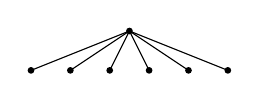
\begin{tikzpicture}[scale=.5]
		\draw(-2.5,0)--(0,1)--(2.5,0);\draw(-1.5,0)--(0,1)--(1.5,0);\draw(-.5,0)--(0,1)--(.5,0);
		\filldraw(-2.5,0)circle(2pt)(2.5,0)circle(2pt)(-1.5,0)circle(2pt)(1.5,0)circle(2pt)(-.5,0)circle(2pt)(.5,0)circle(2pt)(0,1)circle(2pt);
	\end{tikzpicture}&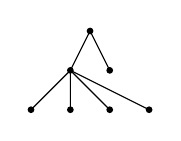
\begin{tikzpicture}[scale=.5]
		\draw(-1.5,0)--(-.5,1)--(1.5,0);\draw(-.5,0)--(-.5,1)--(0,2)--(.5,1);\draw(.5,0)--(-.5,1);
		\filldraw(.5,1)circle(2pt)(0,2)circle(2pt)(-1.5,0)circle(2pt)(1.5,0)circle(2pt)(-.5,0)circle(2pt)(.5,0)circle(2pt)(-.5,1)circle(2pt);
	\end{tikzpicture}&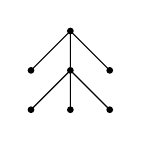
\begin{tikzpicture}[scale=.5]
		\draw(-1,0)--(0,1)--(0,2)--(1,1);\draw(0,2)--(-1,1);\draw(0,0)--(0,1)--(1,0);
		\filldraw(-1,0)circle(2pt)(0,0)circle(2pt)(1,0)circle(2pt)(-1,1)circle(2pt)(0,1)circle(2pt)(1,1)circle(2pt)(0,2)circle(2pt);
	\end{tikzpicture}
	\\
	\{1, 1, 1, 1, 1, 1, 6\}&\{1, 1, 1, 1, 1, 2, 5\}&\{1, 1, 1, 1, 1, 3, 4\}
	\\
	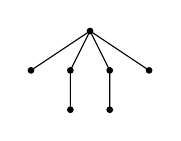
\begin{tikzpicture}[scale=.5]
		\draw(-1.5,1)--(0,2)--(1.5,1);\draw(-.5,0)--(-.5,1)--(0,2)--(.5,1)--(.5,0);
		\filldraw(0,2)circle(2pt)(-1.5,1)circle(2pt)(-.5,1)circle(2pt)(.5,1)circle(2pt)(1.5,1)circle(2pt)(-.5,0)circle(2pt)(.5,0)circle(2pt);
	\end{tikzpicture}&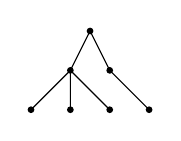
\begin{tikzpicture}[scale=.5]
		\draw(-1.5,0)--(-.5,1)--(0,2)--(.5,1)--(1.5,0);\draw(-.5,0)--(-.5,1)--(.5,0);
		\filldraw(0,2)circle(2pt)(-1.5,0)circle(2pt)(-.5,0)circle(2pt)(.5,0)circle(2pt)(1.5,0)circle(2pt)(-.5,1)circle(2pt)(.5,1)circle(2pt);
	\end{tikzpicture}&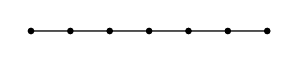
\begin{tikzpicture}[scale=.5]
		\filldraw(-3,0)circle(2pt)--(-2,0)circle(2pt)--(-1,0)circle(2pt)--(0,0)circle(2pt)--(1,0)circle(2pt)--(2,0)circle(2pt)--(3,0)circle(2pt);
	\end{tikzpicture}
	\\
	\{1, 1, 1, 1, 2, 2, 4\}&\{1, 1, 1, 1, 2, 2, 4\}&\{1, 1, 2, 2, 2, 2, 2\}
	\\
	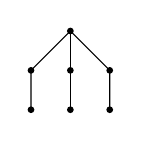
\begin{tikzpicture}[scale=.5]
		\draw(-1,0)--(-1,1)--(0,2)--(1,1)--(1,0);\draw(0,0)--(0,1)--(0,2);
		\filldraw(-1,0)circle(2pt)(-1,1)circle(2pt)(0,2)circle(2pt)(1,1)circle(2pt)(1,0)circle(2pt)(0,0)circle(2pt)(0,1)circle(2pt);
	\end{tikzpicture}&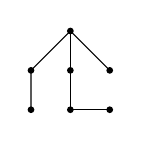
\begin{tikzpicture}[scale=.5]
		\draw(-1,0)--(-1,1)--(0,2)--(1,1);\draw(0,2)--(0,1)--(0,0)--(1,0);
		\filldraw(-1,0)circle(2pt)(-1,1)circle(2pt)(0,2)circle(2pt)(1,1)circle(2pt)(1,0)circle(2pt)(0,0)circle(2pt)(0,1)circle(2pt);
	\end{tikzpicture}&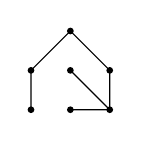
\begin{tikzpicture}[scale=.5]
		\draw(-1,0)--(-1,1)--(0,2)--(1,1)--(1,0)--(0,0);\draw(1,0)--(0,1);
		\filldraw(-1,0)circle(2pt)(-1,1)circle(2pt)(0,2)circle(2pt)(1,1)circle(2pt)(1,0)circle(2pt)(0,0)circle(2pt)(0,1)circle(2pt);
	\end{tikzpicture}
	\\
	\{1, 1, 1, 2, 2, 2, 3\}&\{1, 1, 1, 2, 2, 2, 3\}&\{1, 1, 1, 2, 2, 2, 3\}
	\end{array}\]\[\begin{array}{cc}
	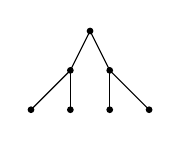
\begin{tikzpicture}[scale=.5]
		\draw(-1.5,0)--(-.5,1)--(0,2)--(.5,1)--(1.5,0);\draw(-.5,1)--(-.5,0);\draw(.5,1)--(.5,0);
		\filldraw(0,2)circle(2pt)(-1.5,0)circle(2pt)(-.5,0)circle(2pt)(1.5,0)circle(2pt)(.5,0)circle(2pt)(-.5,1)circle(2pt)(.5,1)circle(2pt);
	\end{tikzpicture}&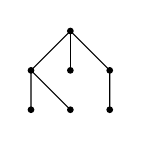
\begin{tikzpicture}[scale=.5]
		\draw(-1,0)--(-1,1)--(0,2)--(1,1)--(1,0);\draw(0,0)--(-1,1);\draw(0,2)--(0,1);
		\filldraw(-1,0)circle(2pt)(-1,1)circle(2pt)(0,2)circle(2pt)(1,1)circle(2pt)(1,0)circle(2pt)(0,0)circle(2pt)(0,1)circle(2pt);
	\end{tikzpicture}
	\\
	\{1, 1, 1, 1, 2, 3, 3\}&\{1, 1, 1, 1, 2, 3, 3\}
	\end{array}\]

	\newpage

	\newcommand{\crit}{
\begin{tikzpicture}\draw[line cap=round,line width=1pt](.1em,-.1em)--(.3em,-.3em)(-.1em,.1em)--(-.3em,.3em)(-.1em,-.1em)--(-.3em,-.3em)(.1em,.1em)--(.3em,.3em);\draw[white,line cap=round,line width=.4pt](.1em,-.1em)--(.3em,-.3em)(-.1em,.1em)--(-.3em,.3em)(-.1em,-.1em)--(-.3em,-.3em)(.1em,.1em)--(.3em,.3em);\end{tikzpicture}}
	\[\crit\,\,nice\,\,\crit\]
	\newsavebox{\critbox}
	\sbox{\critbox}{
		
\begin{tikzpicture}
			\draw[line cap=round,line width=1pt](.1em,-.1em)--(.3em,-.3em)(-.1em,.1em)--(-.3em,.3em)(-.1em,-.1em)--(-.3em,-.3em)(.1em,.1em)--(.3em,.3em);\draw[white,line cap=round,line width=.4pt](.1em,-.1em)--(.3em,-.3em)(-.1em,.1em)--(-.3em,.3em)(-.1em,-.1em)--(-.3em,-.3em)(.1em,.1em)--(.3em,.3em);
		\end{tikzpicture}
	}
	\pgfmathsetseed{\number\pdfrandomseed}
	\[\begin{tikzpicture}%[remember picture,overlay]
		%\pgfmathrandom
		%\node[rotate=20,scale=10,text opacity=.4]at(current page.center){sample text};
		%\draw(current page.center)\node[rotate=30,scale=10,text opacity=.4]{wazzup nigga};
		%\draw(current page.center)node{\usebox{\critbox}};
		%\foreach\x in{1,...,5}{\pgfmathrandominteger{\myangle}{0}{360}\draw(current page.center)circle(4pt)+(\myangle:4pt)circle(1pt);}
		\foreach\x in{1,...,40}{
			\pgfmathrandominteger{\randw}{-.5\textwidth}{.5\textwidth}
			\pgfmathrandominteger{\randh}{0}{40}
			\pgfmathrandominteger{\randangle}{0}{360}
			\draw(current page.center)+(\randw pt,\randh pt)node[rotate=\randangle]{\usebox{\critbox}};
		}
	\end{tikzpicture}\]

	\newpage


		\newcommand{\threedmath}[3]{
			\pgfmathsetmacro\mytheta{#1}
			\pgfmathsetmacro\myphi{#2}
			\pgfmathsetmacro\myroll{#3}
			\pgfmathsetmacro\mycostheta{cos(\mytheta)}
			\pgfmathsetmacro\mysintheta{sin(\mytheta)}
			\pgfmathsetmacro\mycosphi{cos(\myphi)}
			\pgfmathsetmacro\mysinphi{sin(\myphi)}
			\pgfmathsetmacro\mycosroll{cos(\myroll)}
			\pgfmathsetmacro\mysinroll{sin(\myroll)}
			\pgfmathsetmacro\myxx{\mycostheta*\mycosroll-\mysintheta*\mysinphi*\mysinroll}
			\pgfmathsetmacro\myxy{\mysintheta*\mysinphi*\mycosroll+\mycostheta*\mysinroll}
			\pgfmathsetmacro\myyx{-\mysintheta*\mycosroll-\mycostheta*\mysinphi*\mysinroll}
			\pgfmathsetmacro\myyy{\mycostheta*\mysinphi*\mycosroll-\mysintheta*\mysinroll}
			\pgfmathsetmacro\myzx{-\mycosphi*\mysinroll}
			\pgfmathsetmacro\myzy{\mycosphi*\mycosroll}
		}
		\[\threedmath{168}{26}{0}
			\raisebox{3em}{\begin{tikzpicture}[scale=1.3]
				\pgfmathsetmacro\mythreedx{\myxx+\myyx+\myzx}
				\pgfmathsetmacro\mythreedy{\myxy+\myyy+\myzy}
				\pgfmathsetmacro\myotherx{-\myxx+\myyx+\myzx}
				\pgfmathsetmacro\myothery{-\myxy+\myyy+\myzy}
				\draw[notelectricgreen](\mythreedx em,\mythreedy em)--(\myotherx em,\myothery em);
				\pgfmathsetmacro\mythreedx{\myxx+\myyx+\myzx}
				\pgfmathsetmacro\mythreedy{\myxy+\myyy+\myzy}
				\filldraw(\mythreedx em,\mythreedy em)circle(1pt);
				\pgfmathsetmacro\mythreedx{-\myxx+\myyx+\myzx}
				\pgfmathsetmacro\mythreedy{-\myxy+\myyy+\myzy}
				\filldraw(\mythreedx em,\mythreedy em)circle(1pt);
			\end{tikzpicture}}
			\quad\raisebox{3em}{$\to$}\quad
			\raisebox{2em}{\begin{tikzpicture}[scale=1.3]
				\foreach\indexa in{-1,1}{\foreach\indexb in{-1,1}{
						\pgfmathsetmacro\mythreedx{\myxx*\indexa+\myyx*\indexb+\myzx}
						\pgfmathsetmacro\mythreedy{\myxy*\indexa+\myyy*\indexb+\myzy}
						\ifnum\indexa<0{
							\pgfmathsetmacro\myotherx{-\myxx*\indexa+\myyx*\indexb+\myzx}
							\pgfmathsetmacro\myothery{-\myxy*\indexa+\myyy*\indexb+\myzy}
							\draw[notelectricgreen](\mythreedx em,\mythreedy em)--(\myotherx em,\myothery em);
						}\fi\ifnum\indexb<0{
							\pgfmathsetmacro\myotherx{\myxx*\indexa-\myyx*\indexb+\myzx}
							\pgfmathsetmacro\myothery{\myxy*\indexa-\myyy*\indexb+\myzy}
							\draw[notelectricyellow](\mythreedx em,\mythreedy em)--(\myotherx em,\myothery em);
						}\fi
				}}
				\foreach\indexa in{-1,1}{\foreach\indexb in{-1,1}{
						\pgfmathsetmacro\mythreedx{\myxx*\indexa+\myyx*\indexb+\myzx}
						\pgfmathsetmacro\mythreedy{\myxy*\indexa+\myyy*\indexb+\myzy}
						\filldraw(\mythreedx em,\mythreedy em)circle(1pt);
				}}
			\end{tikzpicture}}
			\quad\raisebox{3em}{$\to$}\quad
			\raisebox{1em}{\begin{tikzpicture}[scale=1.3]
				\foreach\indexa in{-1,1}{\foreach\indexb in{-1,1}{\foreach\indexc in{-1,1}{
						\pgfmathsetmacro\mythreedx{\myxx*\indexa+\myyx*\indexb+\myzx*\indexc}
						\pgfmathsetmacro\mythreedy{\myxy*\indexa+\myyy*\indexb+\myzy*\indexc}
						\ifnum\indexa<0{
							\pgfmathsetmacro\myotherx{-\myxx*\indexa+\myyx*\indexb+\myzx*\indexc}
							\pgfmathsetmacro\myothery{-\myxy*\indexa+\myyy*\indexb+\myzy*\indexc}
							\draw[notelectricgreen](\mythreedx em,\mythreedy em)--(\myotherx em,\myothery em);
						}\fi\ifnum\indexb<0{
							\pgfmathsetmacro\myotherx{\myxx*\indexa-\myyx*\indexb+\myzx*\indexc}
							\pgfmathsetmacro\myothery{\myxy*\indexa-\myyy*\indexb+\myzy*\indexc}
							\draw[notelectricyellow](\mythreedx em,\mythreedy em)--(\myotherx em,\myothery em);
						}\fi\ifnum\indexc<0{
							\pgfmathsetmacro\myotherx{\myxx*\indexa+\myyx*\indexb-\myzx*\indexc}
							\pgfmathsetmacro\myothery{\myxy*\indexa+\myyy*\indexb-\myzy*\indexc}
							\draw[red](\mythreedx em,\mythreedy em)--(\myotherx em,\myothery em);
						}\fi
				}}}
				\foreach\indexa in{-1,1}{\foreach\indexb in{-1,1}{\foreach\indexc in{-1,1}{
						\pgfmathsetmacro\mythreedx{\myxx*\indexa+\myyx*\indexb+\myzx*\indexc}
						\pgfmathsetmacro\mythreedy{\myxy*\indexa+\myyy*\indexb+\myzy*\indexc}
						\filldraw(\mythreedx em,\mythreedy em)circle(1pt);
				}}}
			\end{tikzpicture}}
			\quad\raisebox{3em}{$\to$}\quad
			\begin{tikzpicture}[scale=1.3]
				\foreach\indexa in{-1,1}{\foreach\indexb in{-1,1}{\foreach\indexc in{-1,1}{\foreach\indexd in{1,2}{
						\pgfmathsetmacro\mythreedx{\myxx*\indexa+\myyx*\indexb+\myzx*\indexc}
						\pgfmathsetmacro\mythreedy{\myxy*\indexa+\myyy*\indexb+\myzy*\indexc}
						\ifnum\indexa<0{
							\pgfmathsetmacro\myotherx{-\myxx*\indexa+\myyx*\indexb+\myzx*\indexc}
							\pgfmathsetmacro\myothery{-\myxy*\indexa+\myyy*\indexb+\myzy*\indexc}
							\draw[notelectricgreen](\indexd*\mythreedx em,\indexd*\mythreedy em)--(\indexd*\myotherx em,\indexd*\myothery em);
						}\fi\ifnum\indexb<0{
							\pgfmathsetmacro\myotherx{\myxx*\indexa-\myyx*\indexb+\myzx*\indexc}
							\pgfmathsetmacro\myothery{\myxy*\indexa-\myyy*\indexb+\myzy*\indexc}
							\draw[notelectricyellow](\indexd*\mythreedx em,\indexd*\mythreedy em)--(\indexd*\myotherx em,\indexd*\myothery em);
						}\fi\ifnum\indexc<0{
							\pgfmathsetmacro\myotherx{\myxx*\indexa+\myyx*\indexb-\myzx*\indexc}
							\pgfmathsetmacro\myothery{\myxy*\indexa+\myyy*\indexb-\myzy*\indexc}
							\draw[red](\indexd*\mythreedx em,\indexd*\mythreedy em)--(\indexd*\myotherx em,\indexd*\myothery em);
						}\fi\ifnum\indexd<2{
							\draw[blue](2*\mythreedx em,2*\mythreedy em)--(\indexd*\mythreedx em,\indexd*\mythreedy em);
						}\fi
				}}}}
				\foreach\indexa in{-1,1}{\foreach\indexb in{-1,1}{\foreach\indexc in{-1,1}{\foreach\indexd in{1,2}{
						\pgfmathsetmacro\mythreedx{\myxx*\indexa+\myyx*\indexb+\myzx*\indexc}
						\pgfmathsetmacro\mythreedy{\myxy*\indexa+\myyy*\indexb+\myzy*\indexc}
						\filldraw(\indexd*\mythreedx em,\indexd*\mythreedy em)circle(1pt);
				}}}}
			\end{tikzpicture}
			\quad\raisebox{3em}{$\to\cdots$}\]
			\newcommand{\hypercube}{
				\begin{tikzpicture}[scale=1.3]
					\foreach\indexa in{-1,1}{\foreach\indexb in{-1,1}{\foreach\indexc in{-1,1}{\foreach\indexd in{1,2}{
							\pgfmathsetmacro\mythreedx{\myxx*\indexa+\myyx*\indexb+\myzx*\indexc}
							\pgfmathsetmacro\mythreedy{\myxy*\indexa+\myyy*\indexb+\myzy*\indexc}
							\ifnum\indexa<0{
								\pgfmathsetmacro\myotherx{-\myxx*\indexa+\myyx*\indexb+\myzx*\indexc}
								\pgfmathsetmacro\myothery{-\myxy*\indexa+\myyy*\indexb+\myzy*\indexc}
								\draw[notelectricgreen](\indexd*\mythreedx em,\indexd*\mythreedy em)--(\indexd*\myotherx em,\indexd*\myothery em);
							}\fi\ifnum\indexb<0{
								\pgfmathsetmacro\myotherx{\myxx*\indexa-\myyx*\indexb+\myzx*\indexc}
								\pgfmathsetmacro\myothery{\myxy*\indexa-\myyy*\indexb+\myzy*\indexc}
								\draw[notelectricyellow](\indexd*\mythreedx em,\indexd*\mythreedy em)--(\indexd*\myotherx em,\indexd*\myothery em);
							}\fi\ifnum\indexc<0{
								\pgfmathsetmacro\myotherx{\myxx*\indexa+\myyx*\indexb-\myzx*\indexc}
								\pgfmathsetmacro\myothery{\myxy*\indexa+\myyy*\indexb-\myzy*\indexc}
								\draw[red](\indexd*\mythreedx em,\indexd*\mythreedy em)--(\indexd*\myotherx em,\indexd*\myothery em);
							}\fi\ifnum\indexd<2{
								\draw[blue](2*\mythreedx em,2*\mythreedy em)--(\indexd*\mythreedx em,\indexd*\mythreedy em);
							}\fi
					}}}}
					\foreach\indexa in{-1,1}{\foreach\indexb in{-1,1}{\foreach\indexc in{-1,1}{\foreach\indexd in{1,2}{
							\pgfmathsetmacro\mythreedx{\myxx*\indexa+\myyx*\indexb+\myzx*\indexc}
							\pgfmathsetmacro\mythreedy{\myxy*\indexa+\myyy*\indexb+\myzy*\indexc}
							\filldraw(\indexd*\mythreedx em,\indexd*\mythreedy em)circle(1pt);
					}}}}
				\end{tikzpicture}
			}
			\[\foreach\myangle in{20,10,0,-10,-20}{\threedmath{\myangle}{20}{0}\hypercube}\]
			\[\foreach\myangle in{20,10,0,-10,-20}{\threedmath{\myangle}{10}{0}\hypercube}\]
			\[\foreach\myangle in{20,10,0,-10,-20}{\threedmath{\myangle}{0}{0}\hypercube}\]
			\[\foreach\myangle in{20,10,0,-10,-20}{\threedmath{\myangle}{-10}{0}\hypercube}\]
			\[\foreach\myangle in{20,10,0,-10,-20}{\threedmath{\myangle}{-20}{0}\hypercube}\]

	\newpage


		\newcommand{\flowersnark}[1]{
			\begin{tikzpicture}[thick]
				\pgfmathsetmacro\nminusone{#1-1}
				\foreach\a in{0,1,...,\nminusone}{
					\pgfmathsetmacro\incang{Mod(\a+1,#1)}
					\ifnum0=\incang{
						\draw[blue](360*\a/#1:.8em)--(360*\incang/#1:.8em);
					}\else\ifodd\a{
						\draw[notelectricyellow](360*\a/#1:.8em)--(360*\incang/#1:.8em);
					}\else{
						\draw[red](360*\a/#1:.8em)--(360*\incang/#1:.8em);
					}\fi\fi
					\ifnum0=\incang{
						\draw[red](360*\a/#1:.8em)--(360*\a/#1:1.5em);
					}\else\ifnum0=\a{
						\draw[notelectricyellow](360*\a/#1:.8em)--(360*\a/#1:1.5em);
					}\else{
						\draw[blue](360*\a/#1:.8em)--(360*\a/#1:1.5em);
					}\fi\fi
					\ifnum0=\a{
						\draw[notelectricgreen](360*\a/#1:1.5em)--(360*\a/#1-72/#1:2em);
					}\else{
						\draw[notelectricyellow](360*\a/#1:1.5em)--(360*\a/#1-72/#1:2em);
					}\fi
					\ifnum0=\incang{
						\draw[blue](360*\a/#1:1.5em)--(360*\a/#1+72/#1:2em);
					}\else{
						\draw[red](360*\a/#1:1.5em)--(360*\a/#1+72/#1:2em);
					}\fi
					\ifnum0=\incang{
						\draw[red](-360/#1+72/#1:2em)--(-72/#1:2em);
					}\else\ifodd\a{
						\draw[notelectricyellow](360*\a/#1+72/#1:2em)..controls(360*\a/#1+120/#1+72/#1:3em)and(360*\a/#1+240/#1+72/#1:3em)..(360*\incang/#1+72/#1:2em);
					}\else{
						\draw[blue](360*\a/#1+72/#1:2em)..controls(360*\a/#1+120/#1+72/#1:3em)and(360*\a/#1+240/#1+72/#1:3em)..(360*\incang/#1+72/#1:2em);
					}\fi\fi
					\ifnum0=\incang{
						\draw[notelectricgreen](-360/#1-72/#1:2em)..controls(-240/#1-24/#1:3.5em)and(-120/#1+24/#1:3.5em)..(72/#1:2em);
					}\else\ifodd\a{
						\draw[red](360*\a/#1-72/#1:2em)..controls(360*\a/#1+120/#1-72/#1:3em)and(360*\a/#1+240/#1-72/#1:3em)..(360*\incang/#1-72/#1:2em);
					}\else{
						\draw[blue](360*\a/#1-72/#1:2em)..controls(360*\a/#1+120/#1-72/#1:3em)and(360*\a/#1+240/#1-72/#1:3em)..(360*\incang/#1-72/#1:2em);
					}\fi\fi
				}
				\foreach\a in{0,1,...,\nminusone}{
					\filldraw(360*\a/#1:.8em)circle(.5pt);
					\filldraw(360*\a/#1:1.5em)circle(.5pt);
					\filldraw(360*\a/#1-72/#1:2em)circle(.5pt);
					\filldraw(360*\a/#1+72/#1:2em)circle(.5pt);
				}
			\end{tikzpicture}
		}
		\[\begin{array}{cccc}
			\flowersnark{3}&\flowersnark{5}&\flowersnark{7}&\flowersnark{9}\\
			\flowersnark{11}&\flowersnark{13}&\flowersnark{15}&\flowersnark{17}\\
			\flowersnark{19}&\flowersnark{21}&\flowersnark{23}&\flowersnark{25}
		\end{array}\]
\end{document}
